\chapter{Vlastní algoritmické řešení}
\label{ch:VlastniAlg}

V této kapitole se zaměříme na popis vlastního algoritmu pro detekci systolických vrcholů a odhad srdeční tepové frekvence z fotopletysmografických signálů.

Našim cílem je vytvořit jednoduchý a efektivní algoritmus, který poskytne spolehlivé výsledky pro různé typy PPG signálů.

\section{Předzpracování PPG signálu}
\label{sec:alg_preproc}

\subsection*{Načtení signálů}
\label{sec:alg_load}
% - Záznamy jsou uloženy v různých formátech, proto je nutné je převést do jednotného formátu.
%    - numpy řetězce, int, float, ... do jedné python knihovny.
% - Dovygenerujeme referenční TF z referenčních systolických vrcholů - použijeme stejný algoritmus pro výpočet ref TF jako pro výpočet TF z námi detekovaných vrcholů.
Jelikož pracujeme se dvěma databázemi - \emph{CapnoBase} a \emph{BUT~PPG}, výstupem po načtení signálů jsou dvě odlišné knihovny, které zpracováváme samostatně později.
Obě databáze mají odlišnou strukturu souborů a formát signálů, což vyžaduje samostatný přístup při jejich načítání.

Databáze \emph{CapnoBase} obsahuje signály uložené v \texttt{.mat} souborech.
Z každého souboru načítáme signál PPG, referenční systolické vrcholy a vzorkovací frekvenci~\cite{CapnoBase}.
Navíc si vygenerujeme referenční tepovou frekvenci (TF) z referenčních vrcholů, a to pomocí stejného algoritmu, který později použijeme pro výpočet TF z našich detekovaných vrcholů.
Pro účely čitelnější vizualizace a zpracování ukládáme též identifikátor záznamu, což jsou první čtyři znaky názvu souboru.

Oproti tomu databáze \emph{BUT~PPG} používá formát \acl{WFDB} (\acs{WFDB}) a obsahuje PPG záznamy v \texttt{.dat} a \texttt{.hea} souborech.
Tato databáze původně obsahovala 48 záznamů, které byly později rozšířeny o dalších 3~840 záznamů.
Při načítání bylo nutné zohlednit, že starší PPG signály byly uloženy v jednom kanálu, zatímco ostatní signály byly rozděleny do tří kanálů, odpovídajících třem různým barevným složkám signálu~\cite{BUT_PPG_database}.
Z novějších záznamů jsme jako referenční PPG signál vybrali pouze červenou složku, která nejvíce odpovídá standardnímu PPG signálu.

Výsledkem načtení jsou dvě knihovny, které obsahují dostupná data z~obou databází ve formátu vhodném pro další zpracování.

\subsection*{Rozdělení záznamů}
\label{sec:alg_split}
% - Dlouhé záznamy z CapnoBase můžeme rozdělit na kratší úseky, které budou zpracovány jednotlivě.
%   - Z osmiminutového záznamu vytvoříme 8x 1minutový úsek s 10ti procentním překryvem.
Záznamy v databázi \emph{CapnoBase} jsou dlouhé osm minut.
Tuto délku jsme považovali za nevhodnou pro výpočet tepové frekvence, protože výsledná hodnota TF by mohla být zkreslená kratšími úseky se zvýšenou nebo sníženou TF.
Mohlo by se tedy stát, že referenční a naše tepové frekvence by vykazovaly podobné výsledky, přestože by se v jednotlivých úsecích mohly výrazně lišit.

Proto jsme přistoupili k rozdělení každého dlouhého záznamu na kratší, minutové segmenty, které měly pětiprocentní překryv.
Takový překryv byl zaveden proto, abychom testovali algoritmy na všech vrcholech v záznamu a nedošlo k vynechání některých vrcholů na začátku nebo na konci segmentu.
Navíc takový překryv vyhovoval i proto, že počet oken popsaných v podkapitole~\ref{sec:alg_peaks} se rozšíří pouze o jeden.
Rozdělený signál je znázorněn na obr.~\ref{fig:my-detection}.
Výsledné, 63 sekund dlouhé úseky byly dále považovány za samostatné signály, které byly zpracovány jednotlivě.

\subsection*{Filtrace}
\label{sec:alg_filter}
% - Bandpass filter - Butterworthův filtr - vlastní nastavení.
% - Na konec signál standardizujeme od -1 do 1.
Po načtení a případném rozdělení záznamů následovalo filtrování signálu.
Na filtraci jsme použili pásmový filtr čtvrtého řádu typu Butterworth, jehož parametry jsme nastavili s ohledem na fyziologické vlastnosti PPG signálu.
Dolní mez frekvence byla nastavena na 0,5~Hz (30 úderů za minutu) a horní mez na 3,35~Hz (201 úderů za minutu).
Amplitudová charakteristika filtru je znázorněna na obr.~\ref{fig:my_AFC}.

Tento rozsah byl zvolen tak, aby odstranil velmi pomalé změny v signálu, například dechovou frekvenci. Zároveň tak, aby potlačil vysokofrekvenční šum, který by mohl negativně ovlivnit detekci vrcholů.
V nastavení prahů vycházíme z obecných hraničních hodnot lidské tepové frekvence popsané v kapitole~\ref{sec:STF}.

Samotný Butterworthův filtr byl zvolen pro jeho rovnost v propustném pásmu, takže amplitudová charakteristika filtru je hladká a nevykazuje vlnění, které je typické pro některé jiné typy filtrů.
Čtvrtý řád zajišťuje dostatečný kompromis mezi strmostí přechodu a numerickou stabilitou filtru.
Pro odstranění fázového posunu, který je charakteristický pro použitý filtr, jsme použili nulofázový filtr, jenž provádí filtraci v obou směrech.

\begin{figure}[h]
	\label{fig:my_AFC}
	\centering
	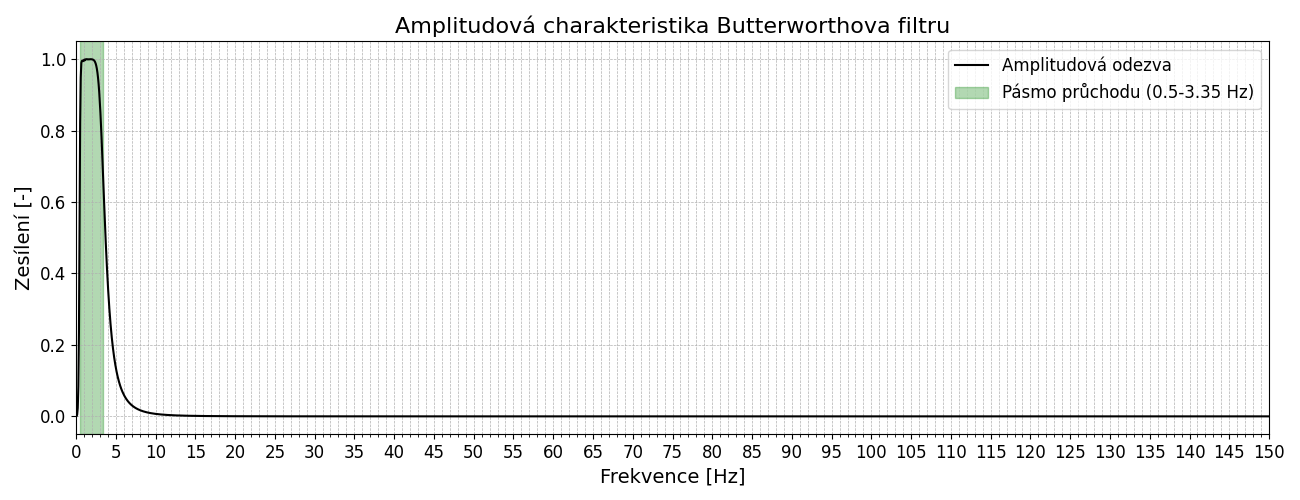
\includegraphics[width=1\textwidth]{./obrazky/My_AFC.png}
	\vspace{-5mm}
	\caption[Vlastní amplitudová charakteristika Butterworthova filtru]{Amplitudová charakteristika Butterworthova filtru.}
	\vspace{-5mm}
\end{figure}

Po filtraci jsme signál standardizovali do rozsahu od \(-1\) do \(1\).
Tato normalizace zajišťuje jednotné měřítko napříč všemi záznamy, což je důležité pro následné kroky detekce, kde algoritmus pracuje s relativními prahy.

Výsledky filtrace a standardizace jsou zřetelné z obr.~\ref{fig:filter-peaks}.
Po těchto krocích jsme získali očištěný a normalizovaný signál, připravený pro detekci systolických vrcholů.

\section{Detekce vrcholů}
\label{sec:alg_peaks}
% - Detekce vrcholů v 5ti sekundových oknech, které se z 50ti procent překrývají.
%   - koukáme na 5 sekund, pak posuneme o 2,5 sekundy a znovu koukáme na dalších 5 sekund.
% - standardizace signálu v okně: -1 do 1 = děláme to znovu
% - nastavení prahů - min_peak_height (lokální brute force 0,3), min_peak_distance (200 bps)
% - lokal max detektor:
%       - koukne na každý vzorek a porovná ho s předchozím a následujícím vzorkem.
%       - pokud je větší než oba AND je větší než nastavené prahy, tak je to vrchol.
% - na konci jen odstraníme vrcholy, které jsou na stejném vzorku (kvůli překrývání oken), protože chceme v budoucnu pracovat i s tím, kolik jsme našli vrcholů v okně - duplikáty by nám to zkreslily.
Hledání vrcholů probíhá v pětisekundových oknech, která se překrývají o 50\%.
Funguje to tak, že nejprve analyzujeme prvních 5 sekund signálu, poté posuneme okno o 2,5 sekundy a analyzujeme dalších 5 sekund, přičemž prvních 2,5 sekund se překrývají s předchozím oknem.
Tímto způsobem pokryjeme celý signál a zajistíme, že žádný vrchol nebude vynechán.
Na jeden minutový úsek obvykle připadá 23 oken, ale protože máme 5\% překryv celého minutového záznamu, délka výsledného signálu je 63 sekund, a proto analyzujeme o jedno okno navíc.
Vizuálně je to znázorněno na obr.~\ref{fig:my-detection}.

Pro celý signál jsme nastavili dva prahy.
První prahová hodnota odpovídala minimální výšce vrcholu, který považujeme za platný.
Tato hodnota byla nastavena na 0,3 a měla za cíl odlišit skutečné vrcholy od diastolických zářezů a šumu.
Druhá prahová hodnota odpovídala minimálnímu časovému intervalu mezi dvěma po sobě jdoucími vrcholy.
To bylo nastaveno na počet vzorků odpovídající 200 tepů za minutu.

\begin{figure} [h]
	\label{fig:my-detection}
	\centering
	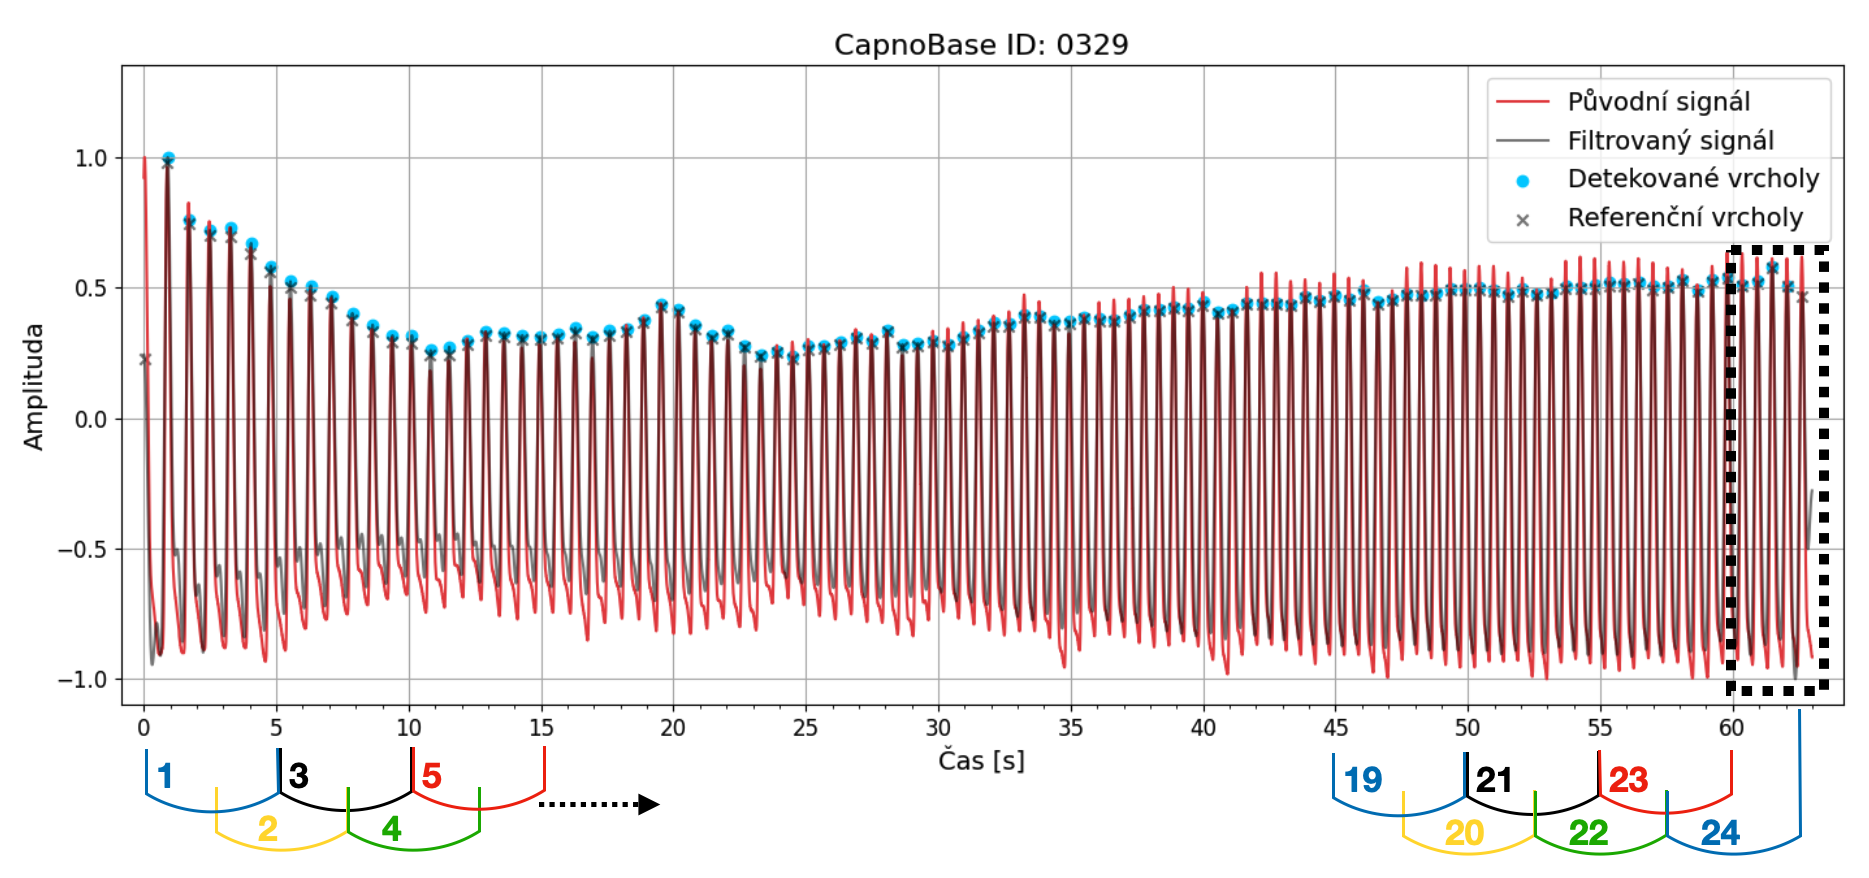
\includegraphics[width=1\textwidth]{./obrazky/My_peaks.png}
	\caption[Vlastní detekce vrcholů]{Druhá minuta záznamu s vizualizací oken a s překryvem.}
\end{figure}

V každém okně jsme provedli standardizaci signálu do rozsahu od \(-1\) do \(1\), abychom zajistili, že nastavené prahy budou co nejpřesněji odpovídat předpokládaným morfologickým vlastnostem PPG signálu.
U signálů jako je zobrazený na obr.~\ref{fig:my-detection} je opětovná standardizace potřebná, protože se amplituda systolické vlny může snižovat a nastavený prah na minimální výšku vrcholu by mohl být příliš nízký, což by vedlo k falešně negativním výsledkům.

Samotná detekce vrcholů je realizována jednoduchým algoritmem hledající lokální maxima.
Funguje tak, že každý vzorek v okně je porovnán se svým předchozím a následujícím sousedem.
Pokud je jeho hodnota větší než hodnota obou sousedů a současně překračuje oba zadané prahy, je tento vzorek označen jako systolický vrchol.

V závěru se odstraní případné duplicitní detekce, které vznikly vlivem překrývání oken.
Vrchol detekovaný na stejném časovém vzorku ve dvou sousedních oknech je ponechán pouze jednou.
Tento krok je důležitý zejména pro budoucí hodnocení algoritmu, kde pracujeme nejen s informací o pozici vrcholů, ale také s jejich počtem v jednotlivých úsecích.
Duplicitní detekce by vedly ke zkreslení metrik a nesprávné interpretaci výsledků.

Posledním krokem je zpětná kontrola minimální vzdálenosti mezi detekovanými vrcholy.
Bez této kontroly by se mohlo stát, že bychom detekovali vrchol na konci prvního okna a u dalšího okna bychom detekovali nový vrchol příliš blízko, protože si nové okno nepamatuje pozici předchozího vrcholu.
Příklad takové chyby je zobrazen na obr.~\ref{fig:filter-peaks}, ve druhém okně.

\section{Výpočet tepové frekvence}
\label{sec:alg_hr}
% - výpočet IBI z detekovaných vrcholů + popsat matematicky IBI
% - výpočet TF z IBI: TF = 60 / median(IBI) OR TF = 60 / mean(IBI) -- my použijeme median protože počítáme, že se v minutovém úseku (nebo desetisekundovém úseku BUT PPG) může objevit nějaký výrazný artefakt, který by nám zkreslil výpočet průměru. Pro delší úseky bychom použili průměr.
% - stejný postup je i pro výpočet ref TF z referenčních vrcholů (viz. \ref{sec:alg_load}) = můžeme porovnat s naším výstupem.
Základní veličinou pro tento výpočet je interval mezi dvěma po sobě následujícími vrcholy, označovaný jako tepový interval - \acs{IBI} (z anglického \uv{Inter-Beat Interval}).
Ten jsme vypočítali tak, že jsme vzali rozdíl mezi časem detekce aktuálního vrcholu a časem detekce předchozího vrcholu:
\begin{equation}
	\label{eq:IBI}
	IBI_{i} = t_{i} - t_{i-1}.
\end{equation}
Výsledkem je sekvence hodnot, které odpovídají časovým intervalům mezi jednotlivými systolickými vrcholy.

Z těchto intervalů jsme odvodili tepovou frekvenci pomocí vztahu popsaném rovnicí (\ref{eq:TF}).
\begin{equation}
	\label{eq:TF}
	TF = \frac{60}{IBI_{median}}
\end{equation}
Po volbě mezi průměrem, mediánem a modusem jsme se rozhodli pro medián.
Na rozdíl od modusové a průměrné hodnoty byl medián nejméně citlivý na extrémní hodnoty, které by mohly zkreslit výpočet průměru.
Na příklad na obr.~\ref{fig:HR_hist} vidíme, jak se může lišit průměr, modus a medián u signálů z našich databází.

\begin{figure}[b]
	\label{fig:HR_hist}
	\centering
	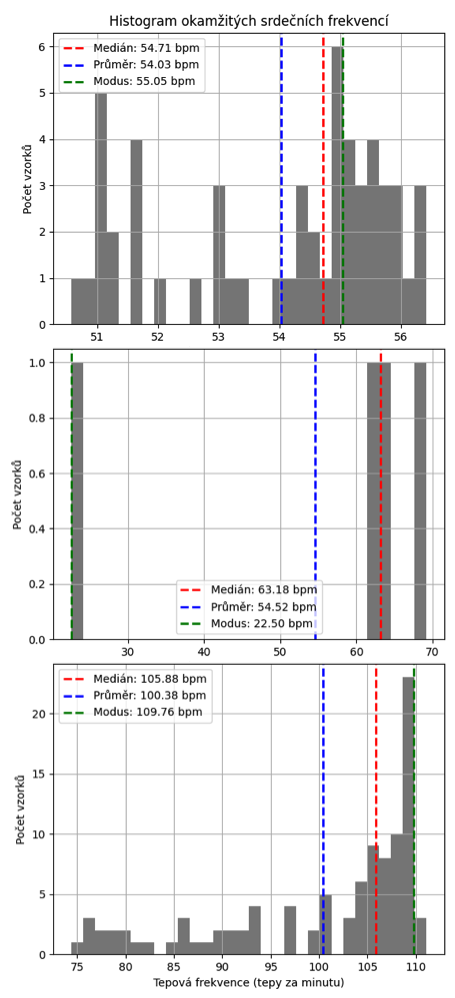
\includegraphics[width=0.7\textwidth]{./obrazky/HR_Hist.png}
	\caption[Histogram IBI]{Stanovení TF z IBI pomocí průměru, mediánu a modusu.}
	\vspace{-5mm}
\end{figure}

\begin{figure}[t]
	\label{fig:filter-peaks}
	\centering
	\vspace{-10mm}
	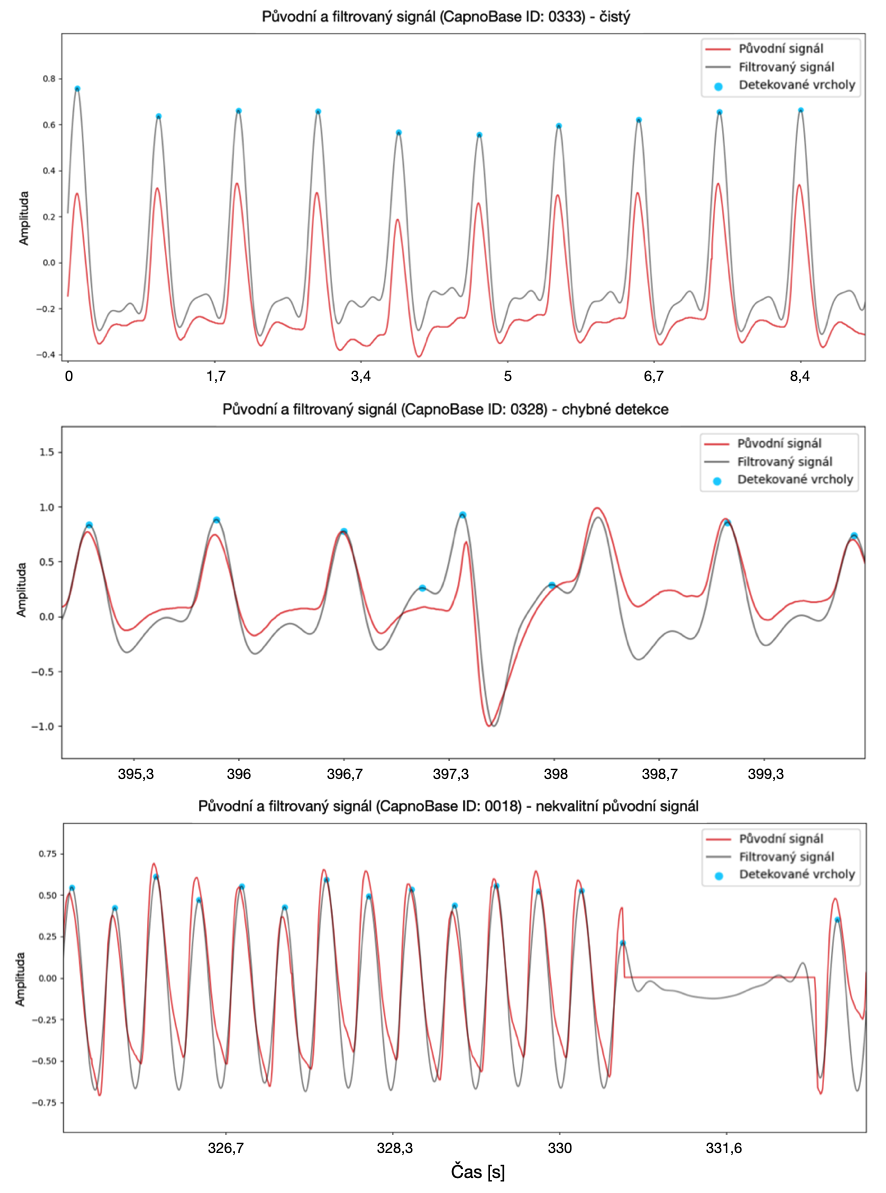
\includegraphics[width=1\textwidth]{./obrazky/MyFilterPeaks.png}
	\caption[Vlastní zpracování signálů]{...}
	\vspace{-15mm}
\end{figure}